\section{Question 1}
We know inertia matrix is symetric so we have:
$$I_{xy} = I_{yx} = 10, \quad I_{xz} = I_{zx} = 0, \quad I_{yz} = I_{zy}$$

$$\boldsymbol{\mathrm{I}} = \begin{bmatrix}
    30 & -10 & 0 \\
    -10 & 20 & -I_{yz}\\
    0 & -I_{yz} & 30
\end{bmatrix}$$
\subsection{part a}
We know that:
\begin{equation}
    \boldsymbol{\mathrm{I}} \times \boldsymbol{\mathrm{\omega}} = \boldsymbol{\mathrm{h}}
\end{equation}

$$
\boldsymbol{\mathrm{\omega}} = \begin{bmatrix}
    10 & 10 & 10
\end{bmatrix}^T_{RPS} = \begin{bmatrix}
    10\times2\pi & 10\times2\pi & 10\times2\pi
\end{bmatrix}^T_{rad/\sec}, \quad \boldsymbol{\mathrm{h}} = \begin{bmatrix}
    200 & 200 & 400
\end{bmatrix}^T_{kg.m^2/s}
$$
If we use radian per second instead of revelotion per second $\boldsymbol{\mathrm{I}} \times \boldsymbol {\mathrm{\omega}} \neq \boldsymbol{\mathrm{h}}$ would happen.
$$ 
\boldsymbol{\mathrm{I}} \times \boldsymbol{\mathrm{\omega}} = \begin{bmatrix}
    200
    \\
    100 - 10I_{yz} \\
    300 - 10I_{yz}
\end{bmatrix} = \begin{bmatrix}
    200\\
    200\\
    400
\end{bmatrix} \rightarrow I_{yz} = -10 \rightarrow 
\boldsymbol{\mathrm{I}} = \begin{bmatrix}
    30 & -10 & 0 \\
    -10 & 20 & 10\\
    0 & 10 & 30
\end{bmatrix}
$$

\begin{equation}
T_{Rotational} = \dfrac{1}{2}\boldsymbol{\mathrm{\omega}}^T\times \boldsymbol{\mathrm{I}} \times \boldsymbol{\mathrm{\omega}} = \dfrac{1}{2} \begin{bmatrix}
    10&
    10&
    10
\end{bmatrix}\times
\begin{bmatrix}
    30 & -10 & 0 \\
    -10 & 20 & 10\\
    0 & 10 & 30
\end{bmatrix}\times
\begin{bmatrix}
    10\\
    10\\
    10
\end{bmatrix} = 4000
\end{equation}
\subsection{part b}
\begin{equation}
    T_{Rotational} = \dfrac{1}{2} \mathrm{I}_{\xi} \omega^2 \rightarrow \mathrm{I}_{\xi} = \dfrac{2T_{Rotational}}{\omega^2} = \dfrac{2\times 4000}{300} = 26.67
\end{equation}

Rotation matrix calculated via eigen vector of inertia matrix (used MATLAB to calculate).
\begin{equation}
    \boldsymbol{\mathrm{A}} = \mathrm{eig}(\boldsymbol{\mathrm{I}}) = \begin{bmatrix}
        -0.4082&   -0.7071&   -0.5774\\
        -0.8165&   -0.0000&    0.5774\\
         0.4082&   -0.7071&    0.5774\\
    \end{bmatrix}
\end{equation}
We know that above matrix shows the direction cosines of the principal axes with the primary body axes. Used MATLAB function (dcm2angle) to calculate euler angles between two corinate system.
$$
\begin{bmatrix}
    \phi\\
    \theta\\
    \psi 
\end{bmatrix} = \begin{bmatrix}
  \ang{45.00}\\
  \ang{35.26}\\
  \ang{-120.00}
\end{bmatrix}
$$

\subsection{part c}
Ellipsoid of inertia calculated as folow:
\begin{equation}
    \dfrac{X^2}{\left(\sqrt{\dfrac{1}{\mathrm{I}_x}}\right)^2} + 
    \dfrac{Y^2}{\left(\sqrt{\dfrac{1}{\mathrm{I}_y}}\right)^2} + 
    \dfrac{Z^2}{\left(\sqrt{\dfrac{1}{\mathrm{I}_z}}\right)^2} = 1
\end{equation} 

\begin{figure}[H]
    \caption{elipsoid of inertia}
    \centering
    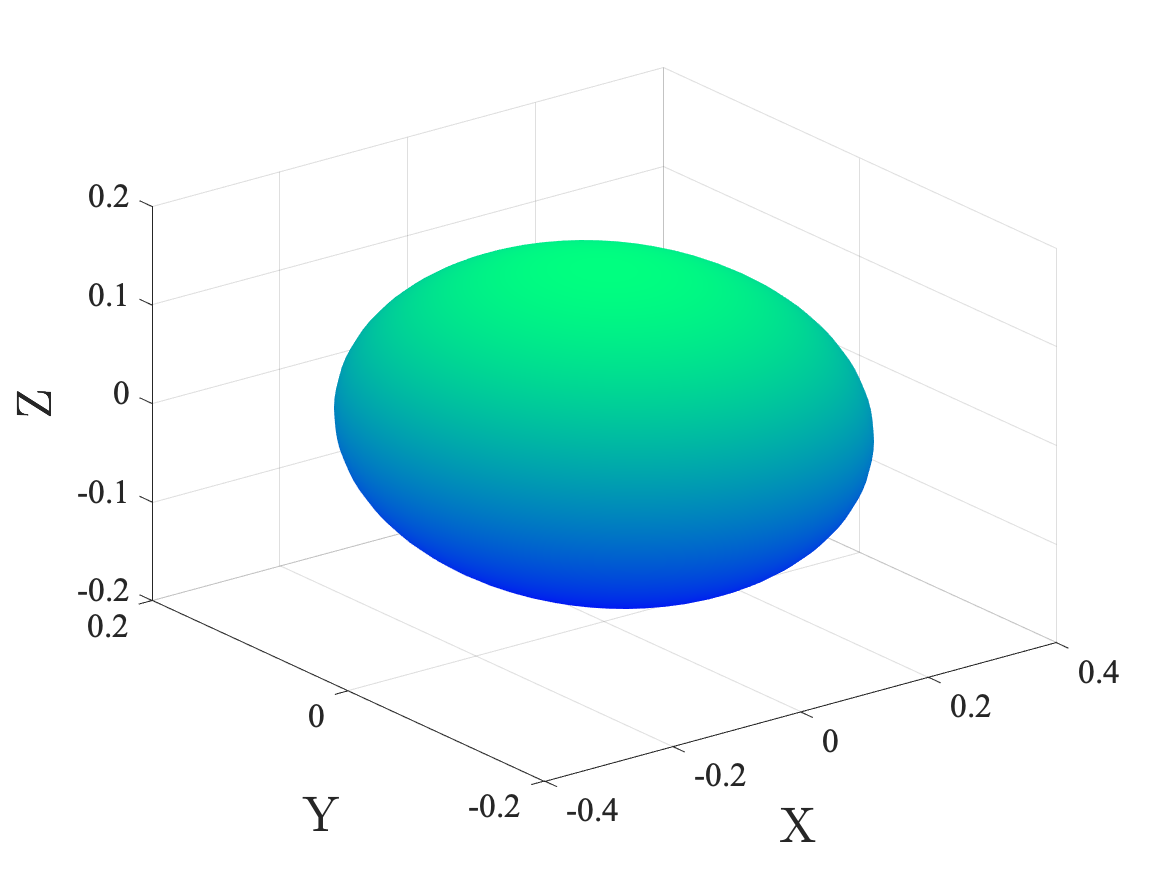
\includegraphics[width=17cm]{../Figure/Q1/3Dof_view_elipsoid_inertia}
\end{figure}

\begin{figure}[H]
    \caption{elipsoid of inertia in zx plane}
    \centering
    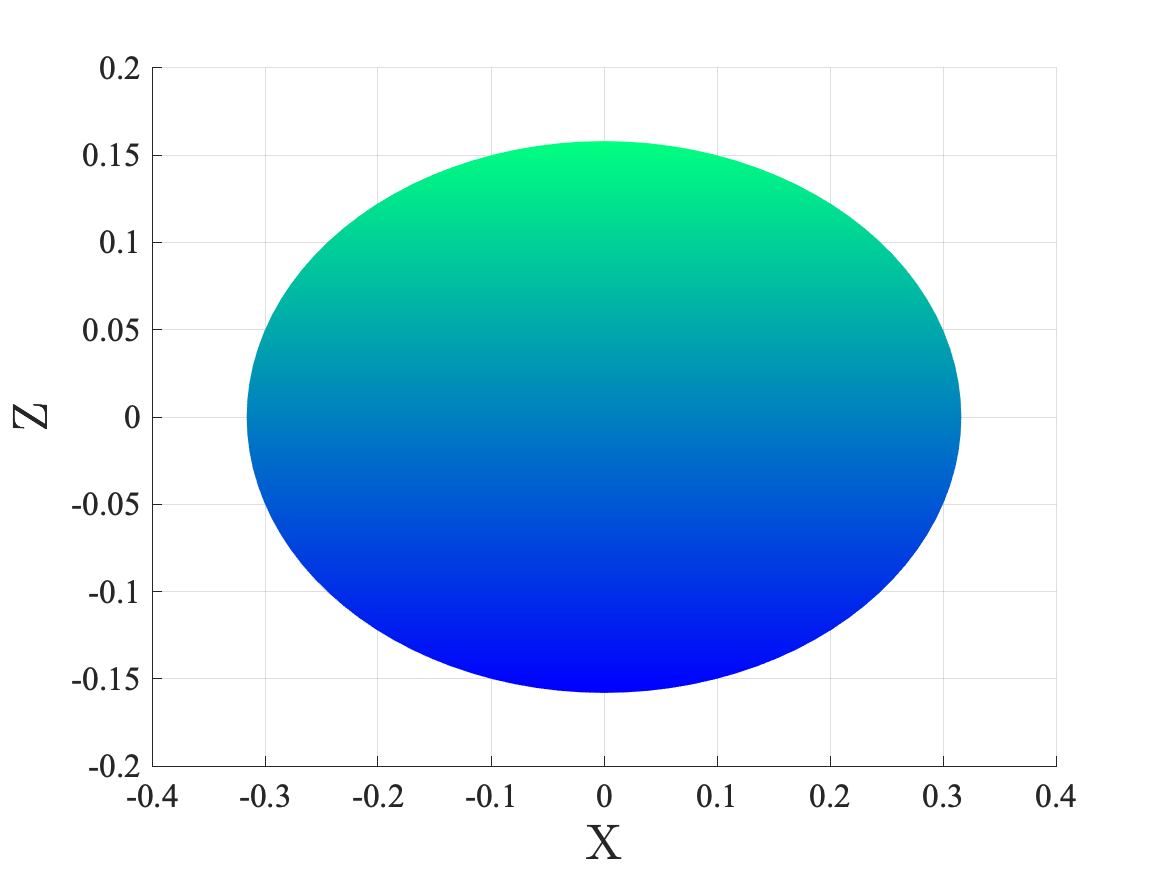
\includegraphics[width=12cm]{../Figure/Q1/xz_view_elipsoid_inertia}
\end{figure}

\begin{figure}[H]
    \caption{elipsoid of inertia zy plane}
    \centering
    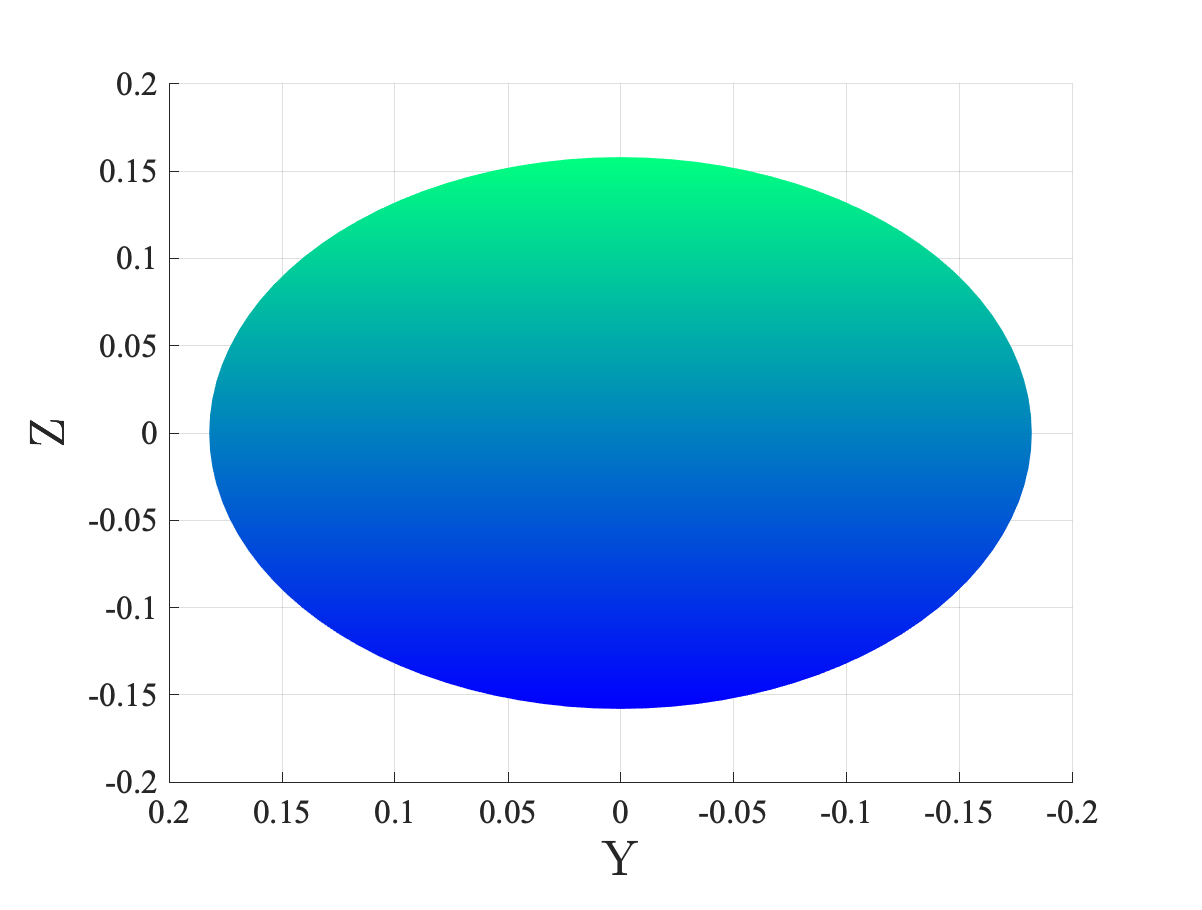
\includegraphics[width=12cm]{../Figure/Q1/yz_view_elipsoid_inertia}
\end{figure}

\begin{figure}[H]
    \caption{elipsoid of inertia in xy plane}
    \centering
    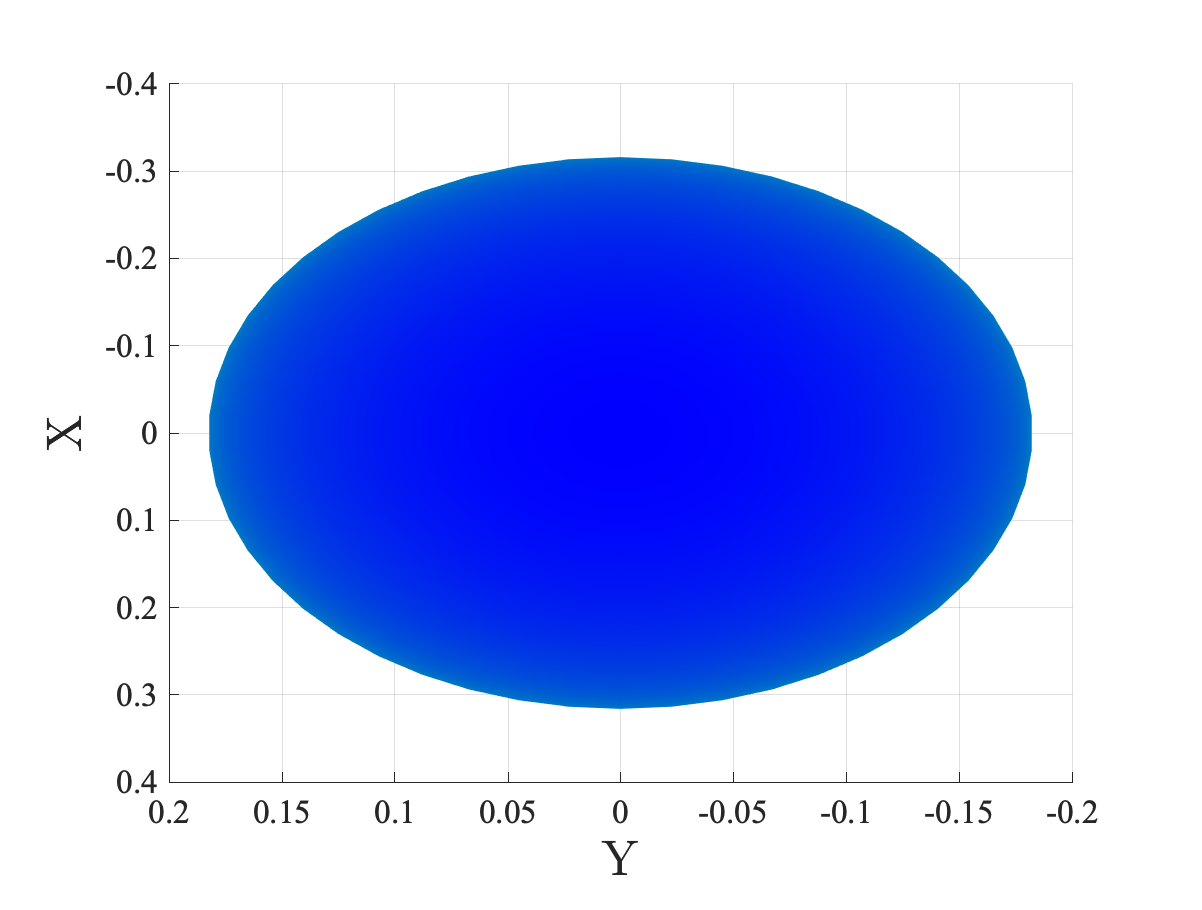
\includegraphics[width=12cm]{../Figure/Q1/xy_view_elipsoid_inertia}
\end{figure}